\input{../documents-common/preamble.tex}
\usepackage[framed]{mcode}
%\usepackage{listings} % Include the listings-package
\begin{document}
\maketitle[Finite Element Methods]{Assignment 2}

\section{}
Start with
\begin{align}
  -\int_\Omega \left[\nabla\cdot\left(\kappa\nabla u\right)\right]v\,\d\vec x &= \int_\Omega fv\,\d\vec x\nn
\end{align}
And then use Green's Theorem (specifically, equation 4.3 from the book) and simplify to find:
\begin{align}
  \int_\Omega \kappa \nabla u \cdot \nabla v\,\d\vec x - \int_{\partial\Omega}\vec n\cdot\left(\kappa\nabla u\right)v\,\d s &= \int_\Omega fv \,\d\vec x\nn
  \int_\Omega \kappa \nabla u \cdot \nabla v \,\d\vec x - \int_{\partial\Omega}\gamma\left(g-u\right)v\,\d s &= \int_\Omega fv \,\d\vec x\nn
  \int_\Omega \kappa \nabla u \cdot \nabla v\,\d\vec x + \int_{\partial\Omega}\gamma uv\,\d s &= \int_\Omega fv\,\d\vec x + \int_{\partial\Omega}\gamma gv\,\d s \nn
\end{align}

\section{}
We compute the AK (and bK) elements using the following code
\lstinputlisting{./code/create_AK_bK.m}

We then compute the eigenvalues of the reference triangle by explicily passing its vertices, using the following function
\lstinputlisting{./code/problem_02.m}

We find that one of the eigenvalues is indeed 0.
\section{}
We have solved problem 3 using the following code, it automatically generates all the necessary plots (formatting was done afterwards).
\lstinputlisting{./code/problem_03.m}
\subsection{}
We have solved the system with the known solution, the result is presented in figure \ref{fig:3a}.
\begin{figure}[!Hh]
  \centering
  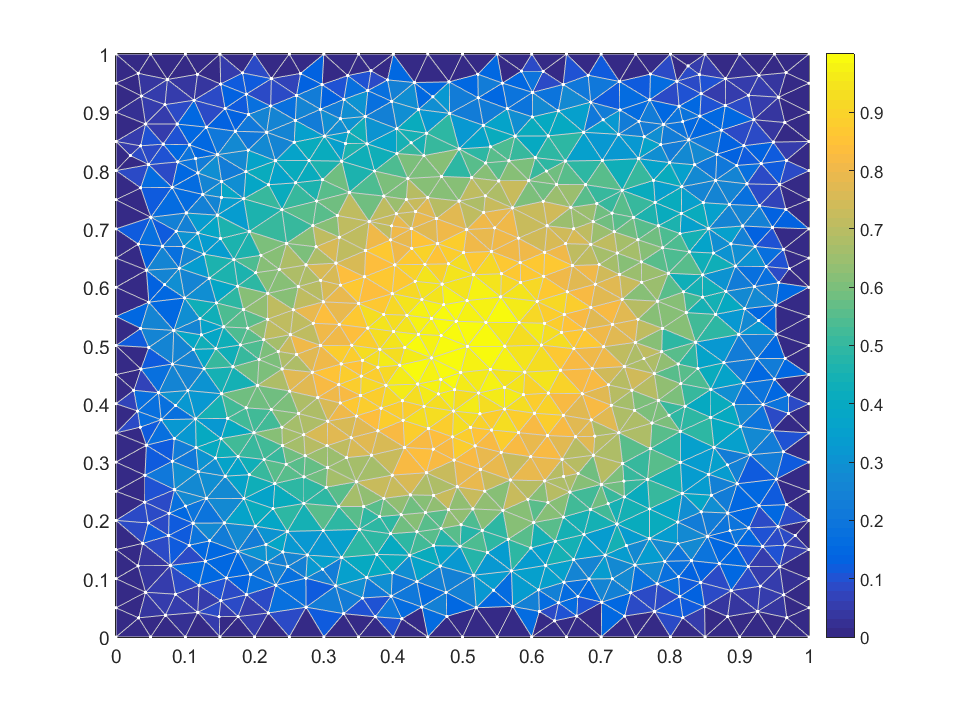
\includegraphics[width=\textwidth]{./plots/problem_03_result}
  \caption{The solution to $-\Delta u = 2\pi^2\sin(\pi x)\sin(\pi y)$ with a zero-boundary.}
  \label{fig:3a}
\end{figure}
\subsection{}
In figure \ref{fig:3b} we have plotted the convergence of the energy-norm in log-log space. The best line fit has a slope of $2.3$ showing the expected 2nd order convergence of our method.
\begin{figure}[!Hh]
  \centering
  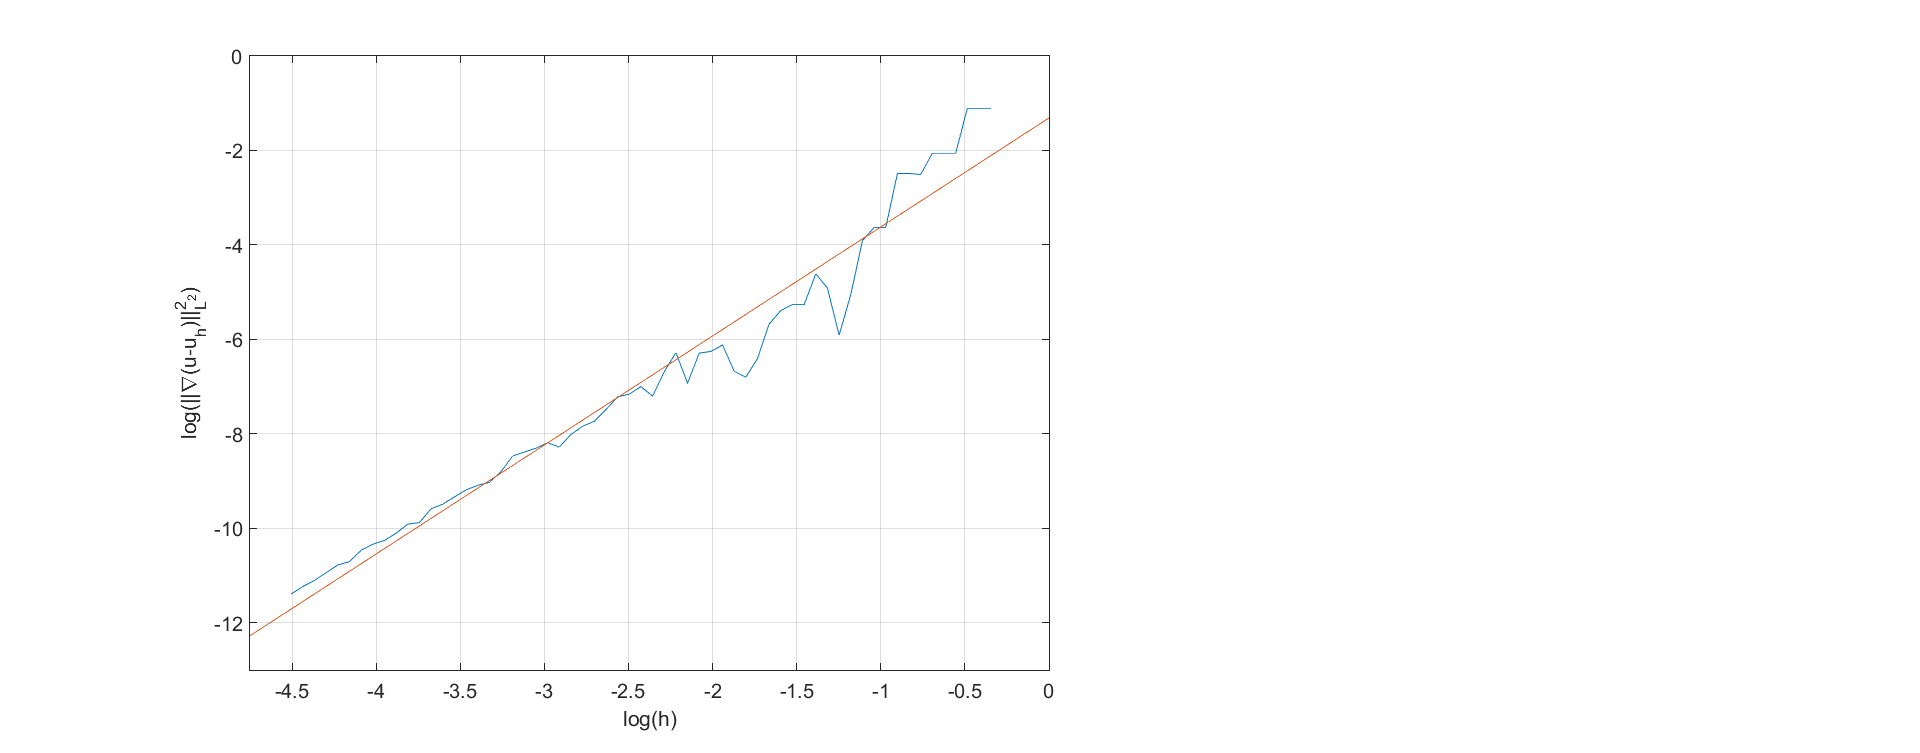
\includegraphics[width=1.5\textwidth]{./plots/problem_03_convergence}
  \caption{Convergence of the energy norm in log-log space. The slope of the best fit is $\approx 2$ showing 2nd-order convergence.}
  \label{fig:3b}
\end{figure}

\section{}
\lstinputlisting{./code/problem_04.m}
We have solved the system with $-\Delta u = 1$ and boundary condition $u = \cos(2\pi y)$ along the y-axis and $0$ elsewhere, the results are shown in figure \ref{fig:4}.
\begin{figure}[!Hh]
  \centering
  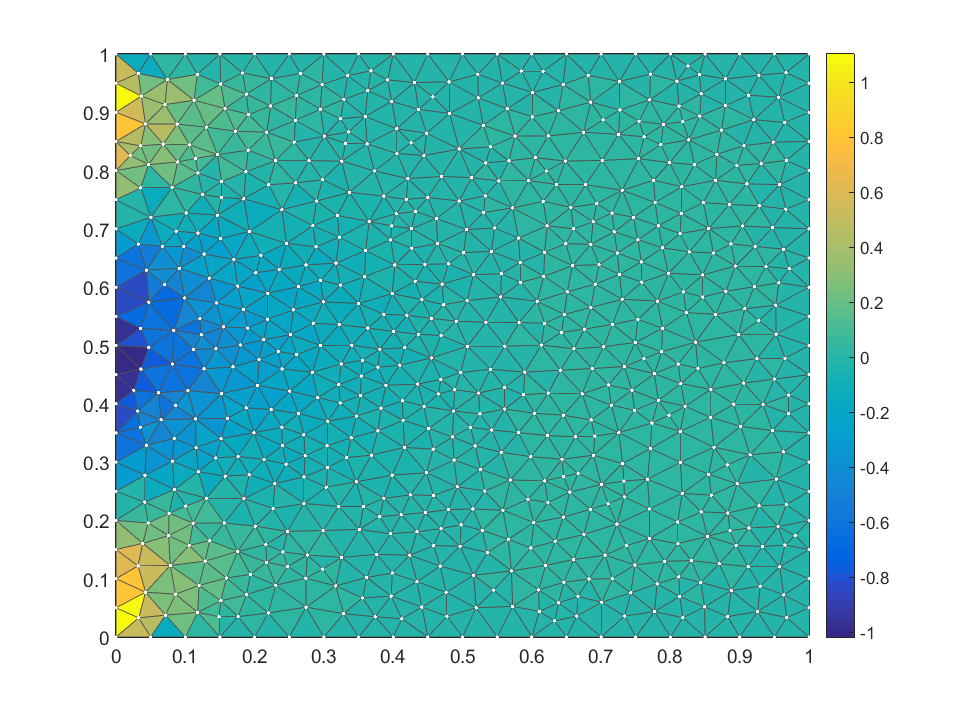
\includegraphics[width=\textwidth]{./plots/problem_04_result}
  \caption{The solution to $-\Delta u = 1$. with boundary condition $u = \cos(2\pi y)$ along the y-axis and $0$ elsewhere.}
  \label{fig:4}
\end{figure}

\end{document}
